\chapter{Method}

\section{Overview}

%seed identification-> short reads collection
The error correction algorithm first collects short reads having the same seed (substrings of length $k$) with each PacBio read. These short reads are aligned onto the PacBio read using a hit-and-extend strategy in conjunction with banded dynamic programming. The errors in each PacBio read, including insertions, deletions, and mismatches, are then replaced with the major alleles in the aligned short reads. In practice, the running time of the above algorithm is unacceptable due to the long length of PacBio reads and huge amount of short reads. The time complexity of each step is listed in Figure~\ref{correction_process}. The following Figure~\ref{correction_process} demonstrates the entire flow of our method, including short reads collection using FM-index, extraction of read sequence, banded dynamic programing, and correction.

\newpage % Overview ended, start a new page to fill figure
\begin{figure}
\centering
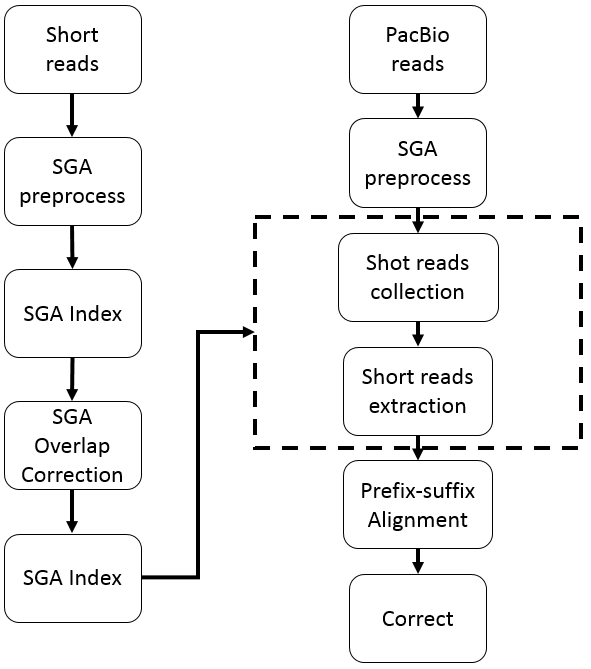
\includegraphics[scale=0.50]{Figures/chapter3/correction_process.png}
\caption{Error correction process}
\label{correction_process}
\end{figure}

\section{Short Reads Collection Using FM-index}


The FM-index of short reads was constructed using Li's ropebwt2 algorithm~\cite{pmid25107872}. Only the short reads sharing common $k$-mer with PacBio reads, which named seed, are considered for correction. The collection of common seeds is done by sliding a $k$-mer window (19 bp by default) along the entire PacBio read. For each $k$-mer in a window, the corresponding suffix array (SA) interval in BWT is computed using the backward search algorithm~\cite{pmid20529929}. In reality, the SA interval within repeats can be very large, and the extraction of each SA index within a repeat interval is extremely slow and less sensitive. In order to reduce the running time, the intervals of per $k$-mer are limited to constant value, which might change due to the coverage, leading to $O(CRk)$ time complexity, where $C$ is the upper limit of SA indices sampled from each SA interval, $R$ is the length of PacBio read and $k$ is the length of a $k$-mer. In our program, $C$ is a used-provided parameter relative to the sequencing coverage. 

\begin{figure} [h]
\centering
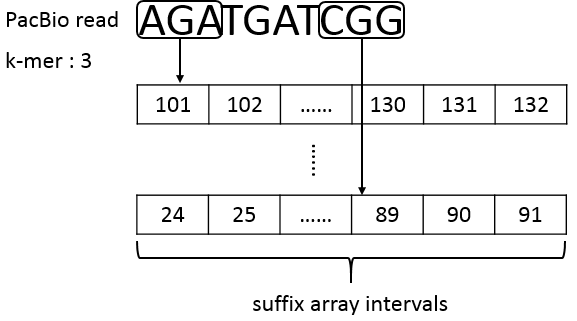
\includegraphics[scale=0.45]{Figures/chapter3/seed_identification.png}
\caption{Example of Short Reads Collection}
\label{Seed_Identification}
\end{figure}


\section{Extraction of Read Sequences from FM-index}

%seed identified-> short reads collected
Each short read having common seed with the PacBio read will be used for correction. However, the short reads collected in previous step only provide implicit SA intervals instead of explicit read sequences, which are required in subsequent pairwise dynamic programming. Therefore, each SA index within the interval needs to be first converted to corresponding read sequence using LF-mapping algorithm~\cite{pmid19261174}. Note that each SA index implies a suffix position within a read. The algorithm has to first backtract from any position to the ending position of the corresponding read (via LF-mapping), and then the sequence can be reconstructed by backtracting from the ending position to the starting position~\cite{pmid20529929}. By assumming the seeds are uniformly distributed in the PacBio read, the expected running time of above algorithm would be $1.5r$, where $r$ is the length of short read.

In order to reduce the time required for backtracting the entire read, we loaded the entire read sequences into memory, which are indexed by read IDs. The above algorithm can thus terminate immediately when backtracting from any suffix position to the ending position, where the read ID can be known and the read sequence can be obtained immediately. This reduces the expected running time from $1.5r$ to $0.5r$, if seeds are uniformly distributed in a PacBio read. Although the entire time complexity is still $O(CRr)$.

\begin{figure} [h]
\centering
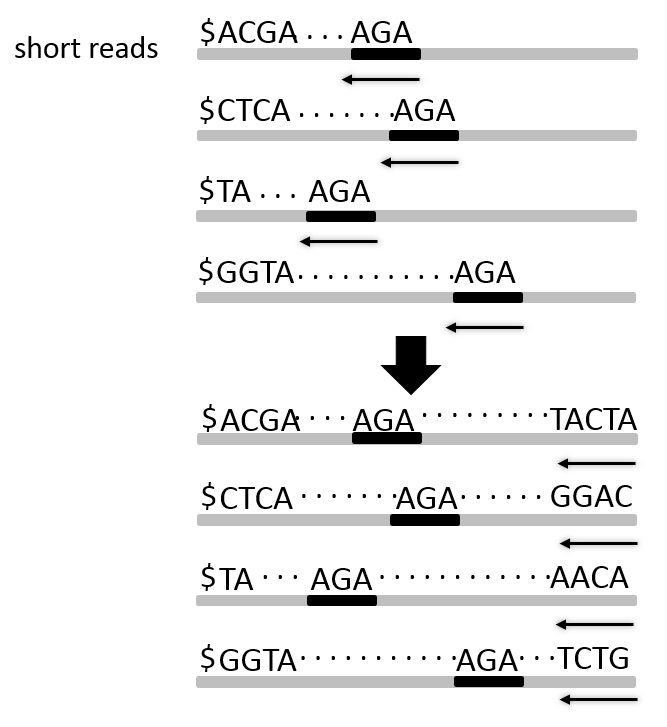
\includegraphics[scale=0.50]{Figures/chapter3/extraction_fm_index.png}
\caption{Extraction by FM-index}
\label{extraction_fm_index}
\end{figure}

\begin{figure} [h]
\centering
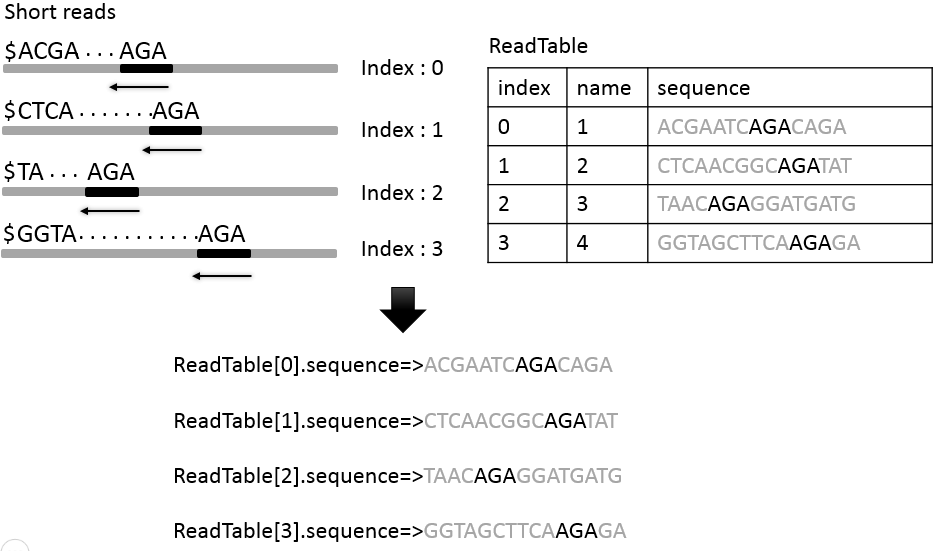
\includegraphics[scale=0.5]{Figures/chapter3/extraction_readtable.png}
\caption{Extraction by readtable}
\label{extraction_readtable}
\end{figure}

\newpage

\section{Prefix-suffix Alignment Using Banded Dynamic Programing}

Each read sequence extracted in previous step is aligned against the PacBio read (sharing common seeds). However, as the PacBio read is rather long ($R>>r$), the original dynamic programming for both reads is rather time-consuming ($O(Rr)$). Because each short read can only be aligned to a small fraction of the PacBio read, the dynamic programming can be further restricted into a smaller fraction surrounding the seed. 


In particular,the total number of insertions and deletions in the alignment is limited to $d-1$ (20 bp by default). Therefore, the alignment should be within the $(d)$ bandwidth centered at the seeding region, and it is unnecessary to compute the lower and upper triangles with respect to the seeding region. We estimate the necessary regions for dynamic programming according to the seed starting positions in PacBio ($P$) and short reads ($p$). The tabular computation can be restricted to $(P-p, P-p+r)$, where $P \geq p$. As a result, the best score of prefix-suffix alignment between these two reads ($S_{i,j}$, where $0 \leq i \leq r$ and $(P-p) \leq j \leq (P-p+r) $) can be computed using the following banded dynamic programming (See figure~\ref{banded_DP_table_with_d3}).
 %or $(0, r-(p-P))$, where $P < p$

\vspace{6pt}
$S_{i,j} = \max \left\{\begin{matrix} S_{i-1, j} - 3 &, insertion\\
S_{i, j-1} - 3 &, deletion\\
S_{i-1, j-1} - 5 &, mismatch\\
S_{i-1, j-1} + 8 &, match \end{matrix}\right\}, 0 \leq i \leq r, (P-p) \leq j \leq (P-p+r)$ 

After finishing the banded DP, we start to trace back at the position $max_{i,j}S(i,j)$ and redo the calculations in the backwards direction to find out where the score came. In other words, from the position $max_{i,j}S(i,j)$, we recalculate $S(i-1,j)$ which is deletion, $S(i-1,j-1)$ which is match or mismatch, and $S(i,j-1)$ which is insertion until the the beginning of baned DP. With the recalculate, we can reconstruct the path that may be with match, mismatch, insertion, deletion (See figure~\ref{Traceback_DP}).


%% This is so confusing. The complexity looks sometimes is all PacBio reads and sometimes only one PacBio read. What exactly are you computing?
For time analysis, note that the area of the $d$ band in the table is $rd$ and the time for filling in every entry inside the band is $O(1)$. In traceback step, the length of the path is approximately $r$ and the time for recalculating in every entry in the path is $O(1)$. Hence, the running time of banded DP algorithm is $O(CRrd)$.

\begin{figure} [h]
\centering
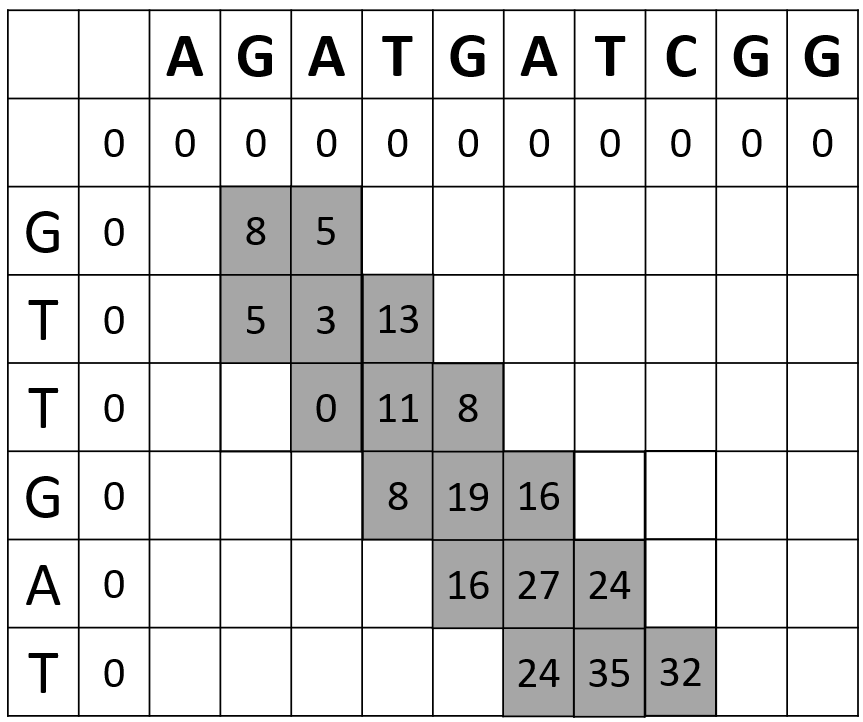
\includegraphics[scale=0.35]{Figures/chapter3/banded_DP_table_with_d3.png}
\caption{An example for banded dynamic programming table with $d=3$}
\label{banded_DP_table_with_d3}
\end{figure}

\begin{figure} [h]
\centering
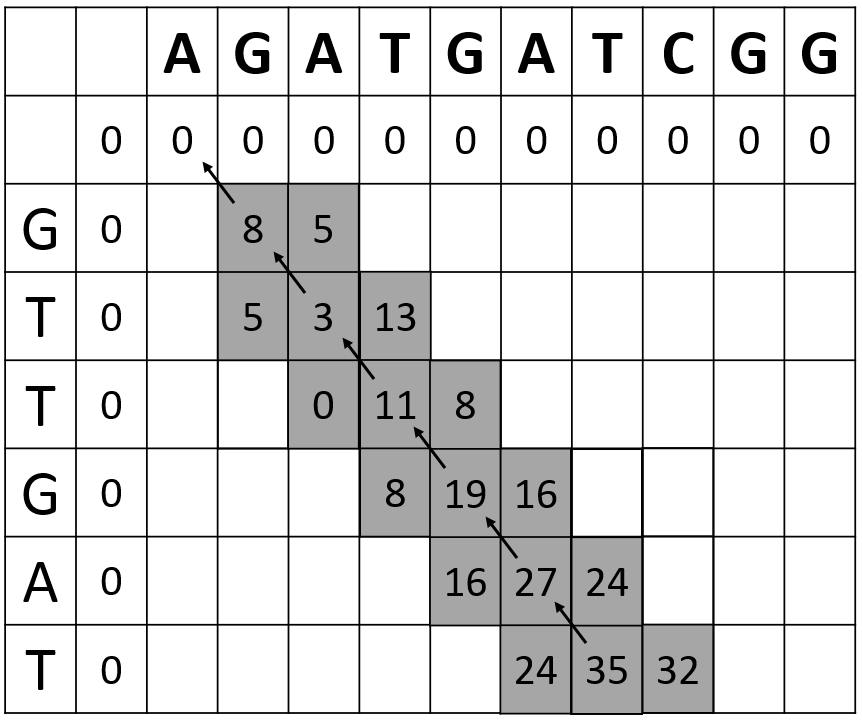
\includegraphics[scale=0.35]{Figures/chapter3/Traceback_DP.png}
\caption{Traceback of banded dynamic programming}
\label{Traceback_DP}
\end{figure}

\newpage

\section{Replacement of Errors by Major Allele}

At this stage, the alleles $(A, T, C, G, -)$ aligned to each base of the PacBio read are known. And the erroneous PacBio allele is replaced with the most-frequent allele (See figure~\ref{replacment}). In reality, there may exist two or more alleles both with high frequencies, owing to SNPs or repeat alleles. If PacBio allele is among the the highest frequency ones, it is retained. Otherwise, it is replaced with arbitrary highest-frequent alleles (if more than one).


Below, we analyze the time complexity of the correction. The time of statistics is $O(CRr)$, where $CR$ is the number of short reads and $r$ is the length of short read. For the replacement, it has to take $O(R)$ to check every position of the PacBio read and extracts elements of each position is $O(1)$. Totally, the time complexity of correction is $O(CRr+R)$

\begin{figure} [h]
\centering
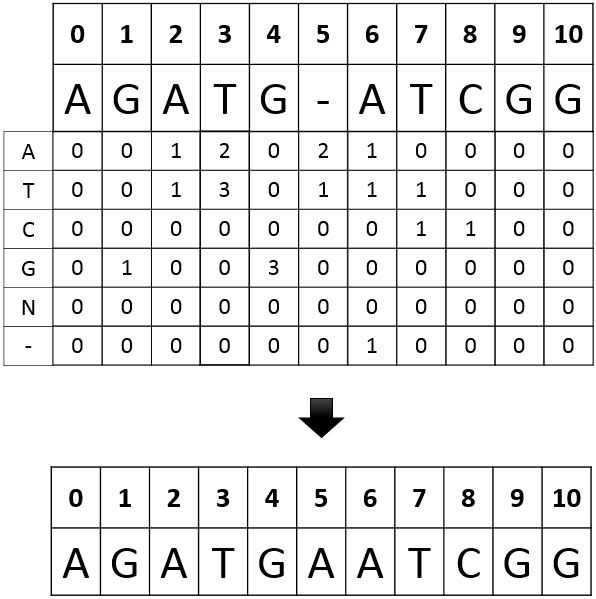
\includegraphics[scale=0.5]{Figures/chapter3/replacmentOfcorrection.png}
\caption{An example of Replacement of Errors by Major Allele}
\label{replacment}
\end{figure}

\newpage

\section{Parallelization}

We tried three parallelization methods including pthread, openMP, and an division-based method in conjunction with openMP. The first is based on Mutex that it will process the thread-number PacBio reads at once time and wait until all threads are finished. In practice, the length of PacBio reads are not uniform so that the running time of processing for each PacBio read is various. The numbers of procedures would wait until the slowest procedure completed at a time. The second separate the procedure into three distinct parts, Reading data from the file, Processing data, and Writing data into the file. Therefore, we have to set critical section lock Reading data from the file and Writing data into the file to avoid race condition and we barely parallel Processing data. In reality, it take too much overhead on critical section, as a result, we figure out the third method that is also based on openMP. Divided-file openMP separates equally the input file and the output file into the numbers of threads. For each thread, it has its own files, which is a input file and a output file, and consequently, we are able to parallel the procedure from reading data to writing data.

\begin{figure} [h]
\centering
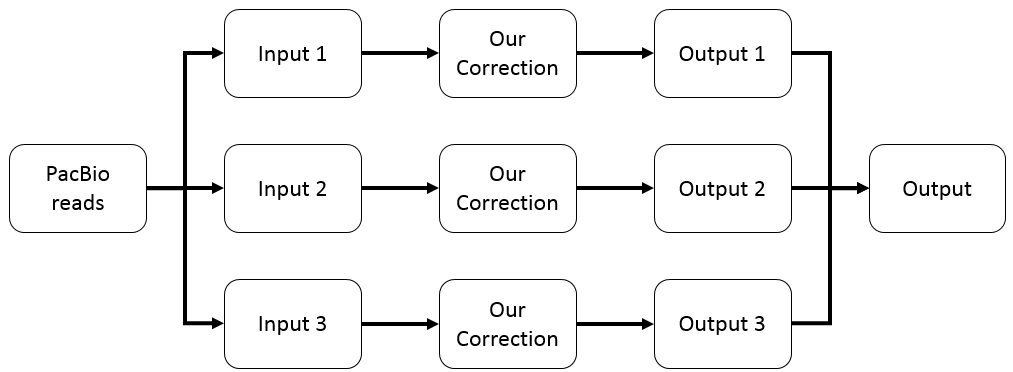
\includegraphics[scale=0.4]{Figures/chapter3/divided_file_openMP.png}
\caption{An example of Divided-file openMP with thread = 3}
\label{divided_file_openMP}
\end{figure}